\documentclass[11pt]{beamer}
\usetheme{simple}
\setbeamertemplate{footline}{} 
\usepackage{tikz}
\usepackage{pgfplots}
\usepackage{amsmath, amssymb, amsthm}   
\pgfplotsset{
        % declare the function you want to plot so you can reuse it easily later
        /pgf/declare function={
            T1(\u)=ln(0.5*(-2*\u+sqrt(4+4*\u^2)));
            T0(\u)=ln(0.5*(2*\u+sqrt(44+4*\u^2)));     
            U0(\u)=\u-1;
            T12(\u)=ln(-1-2*\u);
        },
        % define style to use for the plot to draw only ticks at `\myxlist'
        % (the plot should be invisible)
        my ticks/.style={
            samples at={\myxlist},
            mark=none,
            draw=none,
%            only marks,     % <-- uncomment me to show the data points
        },
every non boxed y axis/.append style={y axis line style=-}
    }
%\pgfplotsset{ every non boxed y axis/.append style={y axis line style=-}}
\setbeamertemplate{navigation symbols}{}
\begin{document}
\begin{frame}
\tikzset{every picture/.style={line width=0.75pt}} %set default line width to 0.75pt        

\begin{tikzpicture}[x=0.75pt,y=0.75pt,yscale=-.8,xscale=.7]
%uncomment if require: \path (0,443); %set diagram left start at 0, and has height of 443
%slide 1


%Shape: Axis 2D [id:dp08487951856920595] 
\draw  (74,382.93) -- (586.09,382.93)(125.21,36.6) -- (125.21,421.41) (579.09,377.93) -- (586.09,382.93) -- (579.09,387.93) (120.21,43.6) -- (125.21,36.6) -- (130.21,43.6)  ;

%Straight Lines [id:da5701690808927993] 
\draw    (127.16,229.64) -- (280.08,229.64) ;


%Straight Lines [id:da9437329096002864] 
\draw    (280.08,386.43) -- (280.08,229.64) ;
\draw [shift={(280.08,229.64)}, rotate = 270] [color={rgb, 255:red, 0; green, 0; blue, 0 }  ][fill={rgb, 255:red, 0; green, 0; blue, 0 }  ][line width=0.75]      (0, 0) circle [x radius= 3.35, y radius= 3.35]   ;

%Shape: Rectangle [id:dp17668651866805996] 
\draw  [draw opacity=0][fill={rgb, 255:red, 74; green, 144; blue, 226 }  ,fill opacity=0.15 ] (127.16,229.64) -- (280.08,229.64) -- (280.08,381) -- (127.16,381) -- cycle ;

% Text Node
\draw (330,213) node   {$( m_{1} ,m_{2})$};

% Text Node
\draw (203.62,305.32) node  [align=left] {\tiny no saving, \\\tiny no borrowing};

\only<2,3>{
%Straight Lines [id:da02010181844261072] 
\draw    (126.3,90) -- (280.08,229.64) ;

%Shape: Right Triangle [id:dp5413850022181785] 
\draw  [draw opacity=0][fill={rgb, 255:red, 74; green, 144; blue, 226 }  ,fill opacity=0.15 ] (126.3,90) -- (280.08,229.64) -- (126.3,229.64) -- cycle ;


%Shape: Right Triangle [id:dp8162358723316316] 
\draw  [draw opacity=0] (126.3,90) -- (280.08,229.64) -- (126.3,229.64) -- cycle ;

% Text Node
\draw (176.62,190.32) node  [align=left] {\tiny saving only};}







\only<3>{
%Straight Lines [id:da7975318034764101] 
\draw    (280.08,229.64) -- (432.3,381.86) ;


%Shape: Right Triangle [id:dp05301219771788945] 
\draw  [draw opacity=0][fill={rgb, 255:red, 74; green, 144; blue, 226 }  ,fill opacity=0.15 ] (280.08,229.64) -- (433.3,383) -- (280.08,383) -- cycle ;


% Text Node
\draw (338.62,350.32) node  [align=left] {\tiny borrowing only};}




% Text Node
\draw (102,231.6) node   {$m_{2}$};
% Text Node
\draw (279,403.6) node   {$m_{1}$};
% Text Node
\draw (597.35,402.33) node   {$x_{1}$};
% Text Node
\draw (105,26.6) node   {$x_{2}$};
% Text Node
\draw (50,88.6) node   {$( 1+r) m_{1} +m_{2}$};
% Text Node
\draw (436,408.6) node   {$m_{1} +\frac{m_{2}}{1+r}$};

\end{tikzpicture}
\end{frame}
\end{document}
